\chapter{Results and Discussions}
In this chapter, the neutron missing mass spectrum of the $^3$He($K^-,n$) reaction is discussed. The spectrum is presented in Sec. \ref{sec-spectrum}. Then, after taking account of the experimental effects and known elementally processes, we find a statistically significant unknown-excess exists just below the $K^-pp$ binding threshold as described in Sec. \ref{sec-excess}. The possible explanations of the unknown excess are discussed in the Sec. \ref{sec-source}. We consider the contributions from two- and three-nucleon absorption processes, and the $K^-pp$ bound state. We also derive upper limits for the formation cross sections of the deeply bound $K^-pp$ state with more than 90 MeV binding energy in Sec. \ref{sec-upper}. 

\section{The obtained neutron spectrum} \label{sec-spectrum}
\subsection{Neutron semi-inclusive spectrum}
Figure \ref{fig-neutron} shows the $1/\beta$ distribution, the neutron momentum distribution and the missing-mass distribution of the $^3$He($K^-,n$) reaction with the final event selection. 
The kaon beam was analyzed and selected as described in Sec. \ref{sec-anabeam}, and the forward neutron momentum was evaluated as given in Sec. \ref{sec-ananc}.

We required at least one charged track reconstructed with the CDS\footnote{Here we did not require an associated hit on the IH.}, and the reconstructed vertex to be inside of the fiducial volume defined as described in Sec. \ref{sec-anacds}. Therefore, the
spectra in Fig. \ref{fig-neutron} are not inclusive ones but somehow distorted by the CDS acceptance of charged-track tagging, $A_{CDS}$, which is limited from 54 to 126 degrees in the polar angle. We call them {\it semi-inclusive } spectra, and thus we should be careful when the spectra are compared with theoretical ones, which are purely inclusive ones in most cases.

\begin{figure}[] 
\begin{center}
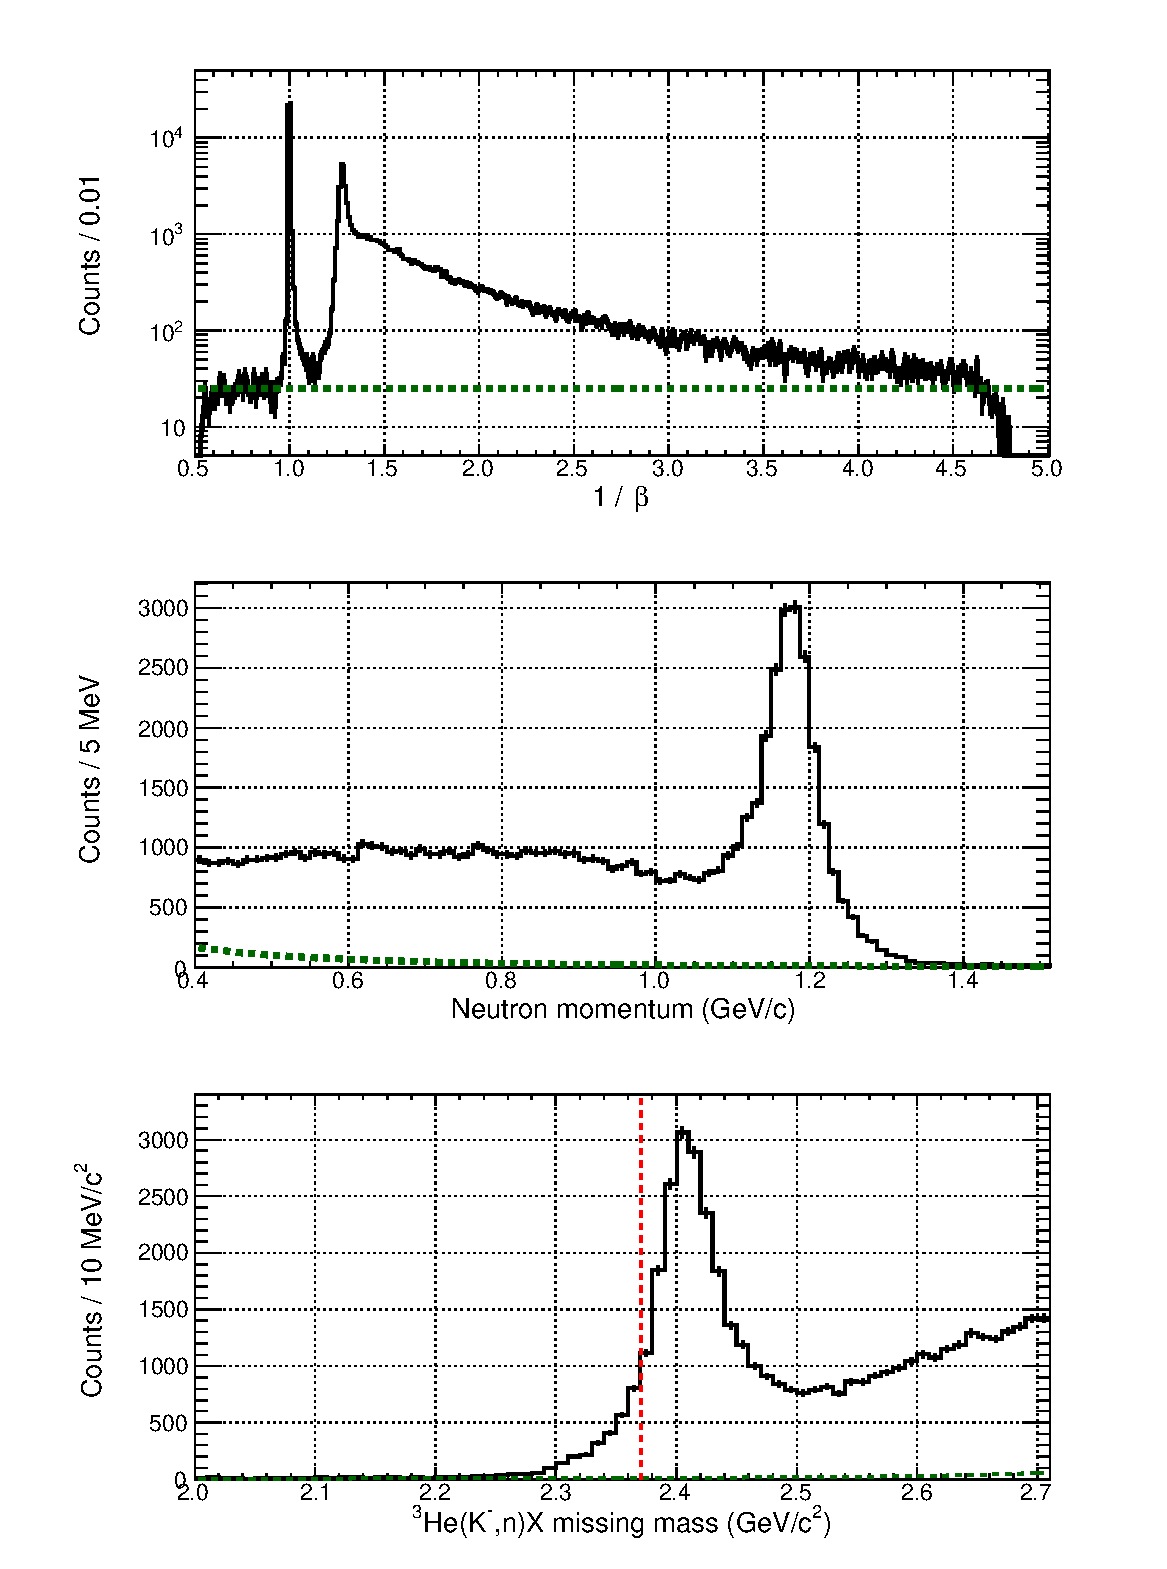
\includegraphics[width=\columnwidth]{./fig/mm-betamommm.eps}
\caption[$1/\beta$ spectrum of the neutral particles, neutron momentum spectrum, and neutron missing-mass spectrum.]{(top) $1/\beta$ spectrum of the neutral particles. The green line represents the accidental background evaluated by fitting the spectrum from 0.6 to 0.9 with a constant function. (middle) Neutron momentum spectrum. (bottom) Neutron missing-mass spectrum. The green lines were analytically converted from that in the 1$/\beta$ spectrum. The red dotted line in the missing mass spectrum represents the $K^-pp$ binding threshold.}
\label{fig-neutron}
\end{center}
\end{figure}  

\subsection{Normalized neutron semi-inclusive spectrum}
Using the normalization factors summarized in Table \ref{tab-ncs}, the normalized missing-mass spectrum of the $^3$He($K^-,n$) reaction at $\theta_{lab} = 0^\circ$ is obtained as shown in Fig. \ref{fig-ncs}. Note that since $A_{CDS}$ depends on each reaction process, the spectrum is not corrected by $A_{CDS}$.
\\


The spectrum shows a clear peak around 2.4 GeV/$c^2$, which is attributed to the quasi-free reactions as expected, however, a certain amount of events is observed as a tail structure below the $K^-pp$ binding threshold.

In the following section, we evaluate contributions in the tail structure of experimental effects, such as the detector resolution and the accidental background, and then investigate whether well-known elementally processes can reproduce the tail structure.

\begin{figure}[]
\begin{center}
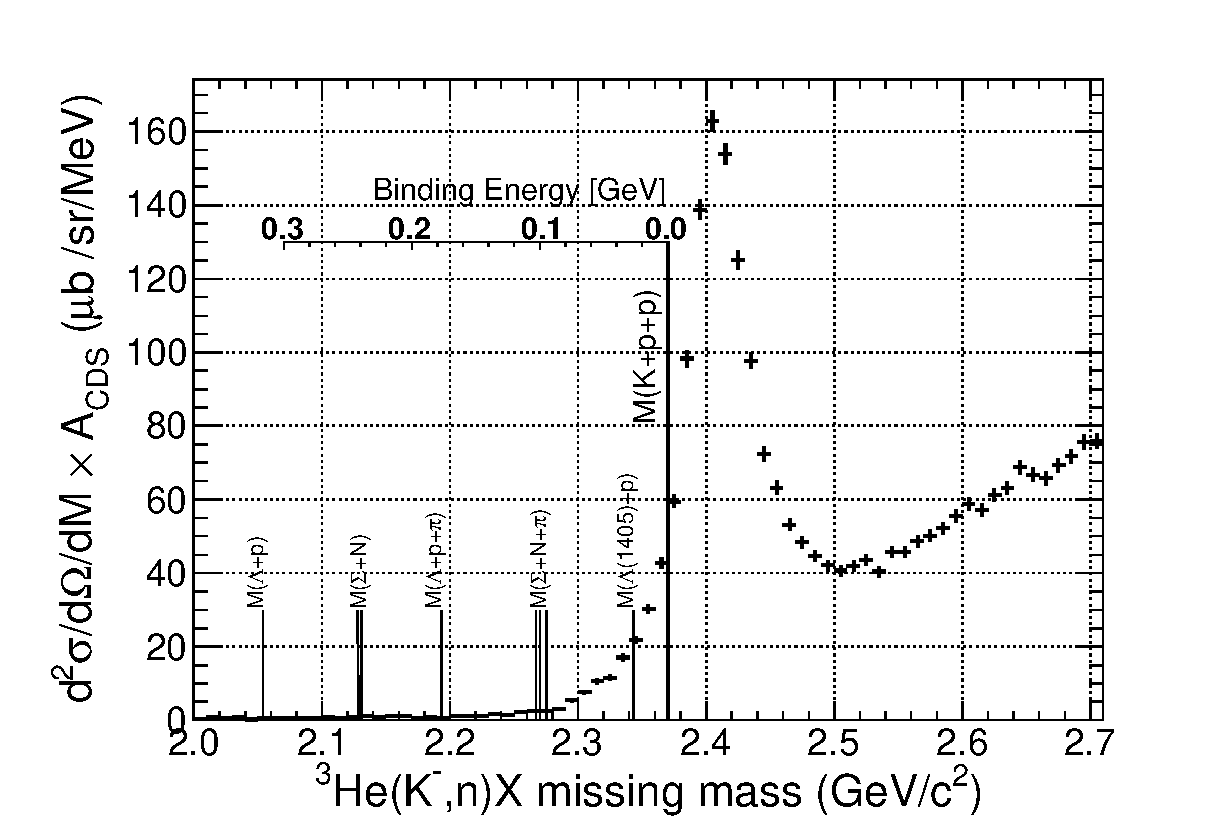
\includegraphics[width=14cm]{./fig/n-cs.eps}
\caption[Normalized neutron spectrum.]{Normalized neutron spectrum. The CDS acceptance of the charged track tagging, $A_{CDS}$, is not corrected.}
\label{fig-ncs}
\end{center}
\end{figure}  

\section{Tail structure below the threshold} \label{sec-excess}
\subsection{Experimental effects} \label{sec-exeff}
\subsubsection{Detector resolution}
To directly show that the tail structure below the threshold is not caused by the experimental resolution, we compared the spectrum with a $K^0_s$-tagged one. Here the $K^0_s\to\pi^+\pi^-$ decays are reconstructed with the CDS and selected as described in Sec. \ref{sec-cdck0}. Figure \ref{fig-nk0tag} shows the comparison between the two spectra. 
The peak structure of the $K^0_s$-tagged spectrum is associated to the charge-exchange reaction,
\begin{eqnarray}
K^- + {\rm ^3He} &\to& K^0 + n + d_s. \label{eq-k0}
\end{eqnarray}
Considering that the spectator nucleus is a deuteron ($d_s$) or a pair of a neutron and a proton, the missing mass of $^3$He($K^-,n)X$ must not be smaller than the sum of the $K^0$ and the deuteron masses, which is almost equivalent to the $K^-+p+p$ mass. The continuum in the $K^0_s$ tagged spectrum is mainly contributed from $\Lambda(1520)$ production via its decay into $K^0_sn$, and $K^0$ production with an associated pion, such as,
\begin{eqnarray}
K^- + {\rm ^3He} &\to& \Lambda(1520)+ \pi^0  + d_s, \label{eq-l1520}\\
&&\Lambda(1520)\to K^0_s + n,\nonumber \\ 
K^- + {\rm ^3He} &\to& K^0 + \pi^0 + n + d_s, \label{eq-k0pi}
\end{eqnarray}
whose missing-mass of $^3$He($K^-,n)X$ should be located at larger than the sum of the pion, the $K^0$ and the deuteron masses.

The $K^0_s$-tagged spectrum actually rises at the $K^-pp$ binding threshold and has few events in the bound region. Therefore, it is the direct evidence that the tail structure cannot be explained by the broadening of the quasi-free peak due to the detector resolution.

\begin{figure}[]
\begin{center}
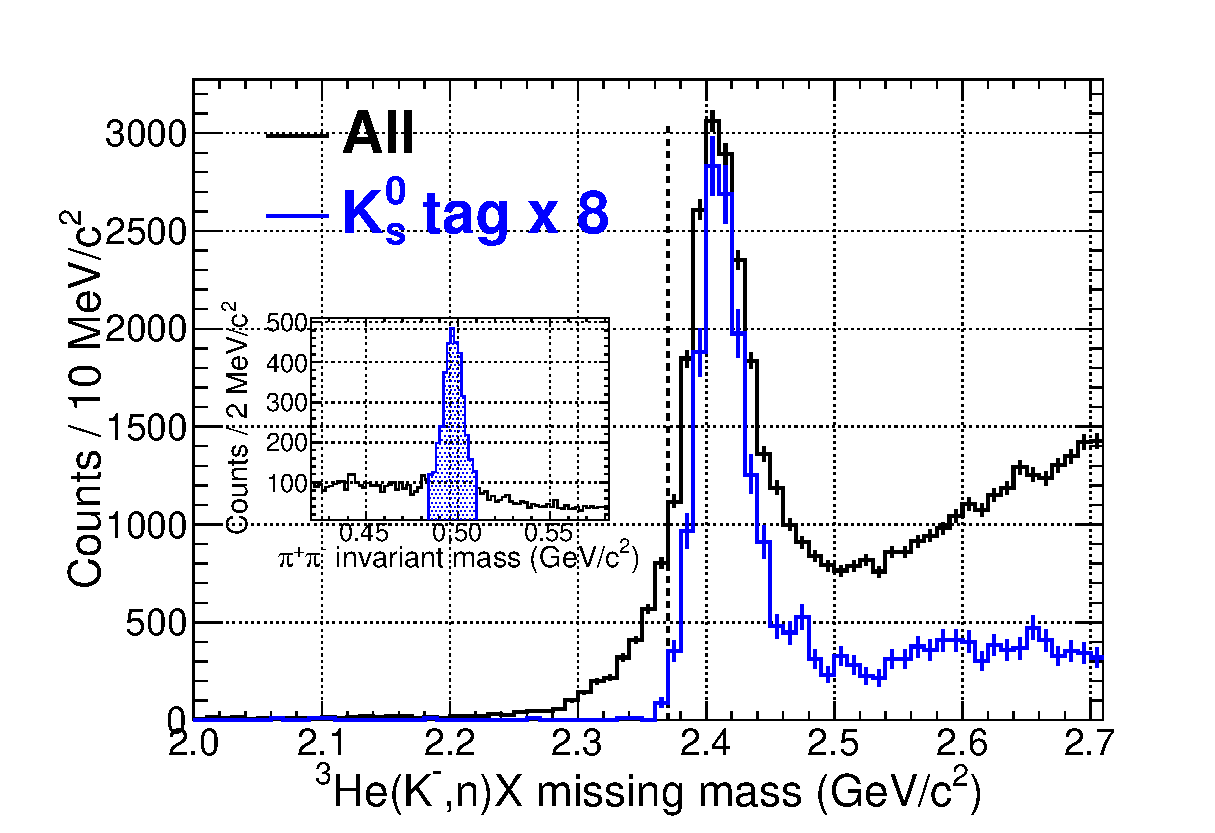
\includegraphics[width=12cm]{./fig/n-k0tag.eps}
\caption[Comparison between the $^3$He($K^-,n)X$ missing-mass and the $K^0_s$-tagged one.]{Comparison between the $^3$He($K^-,n)X$ missing-mass and the $K^0_s$-tagged one. The red histogram represents the $K^0_s$-tagged spectrum with a scale factor of 8. The dotted line represents the $K^-pp$ binding threshold. The inset histogram shows the $K^0_s$ selection region in the $\pi^+\pi^-$ invariant-mass spectrum with a requirement of neutron detection.}
\label{fig-nk0tag}
\end{center}
\end{figure}  

\subsubsection{Contamination from the material around the target}
As shown in Fig. \ref{fig-cdcvertex}, we recorded the production data of not only the $K^-$-$^3$He reaction but also reactions between the kaon and other materials, such as the target cell and the helium transfer pipes. Due to the finite vertex resolution, other reactions than the $K^-$-$^3$He should contaminated in the fiducial-volume selection, especially when the vertex is reconstructed using one charged particle from the $K^0$/$\Lambda$/$\Sigma$ decays. To investigate the contamination, we performed the empty-target run with the same detector setup as the production run.

The empty-target data was analyzed exactly in the same way as the $^3$He run including the vertex selection criteria. The spectrum is compared with the $^3$He data as shown in Fig. \ref{fig-nempty}. The empty-target spectrum is scaled by factor $\sim$10, since the accumulated data was about $\sim$10\% of the production run with $^3$He target on the basis of the number of the incident beam kaon. The contribution from other materials than $^3$He was evaluated to be less than 10\% of $^3$He events in the bound region. 

\begin{figure}[]
\begin{center}
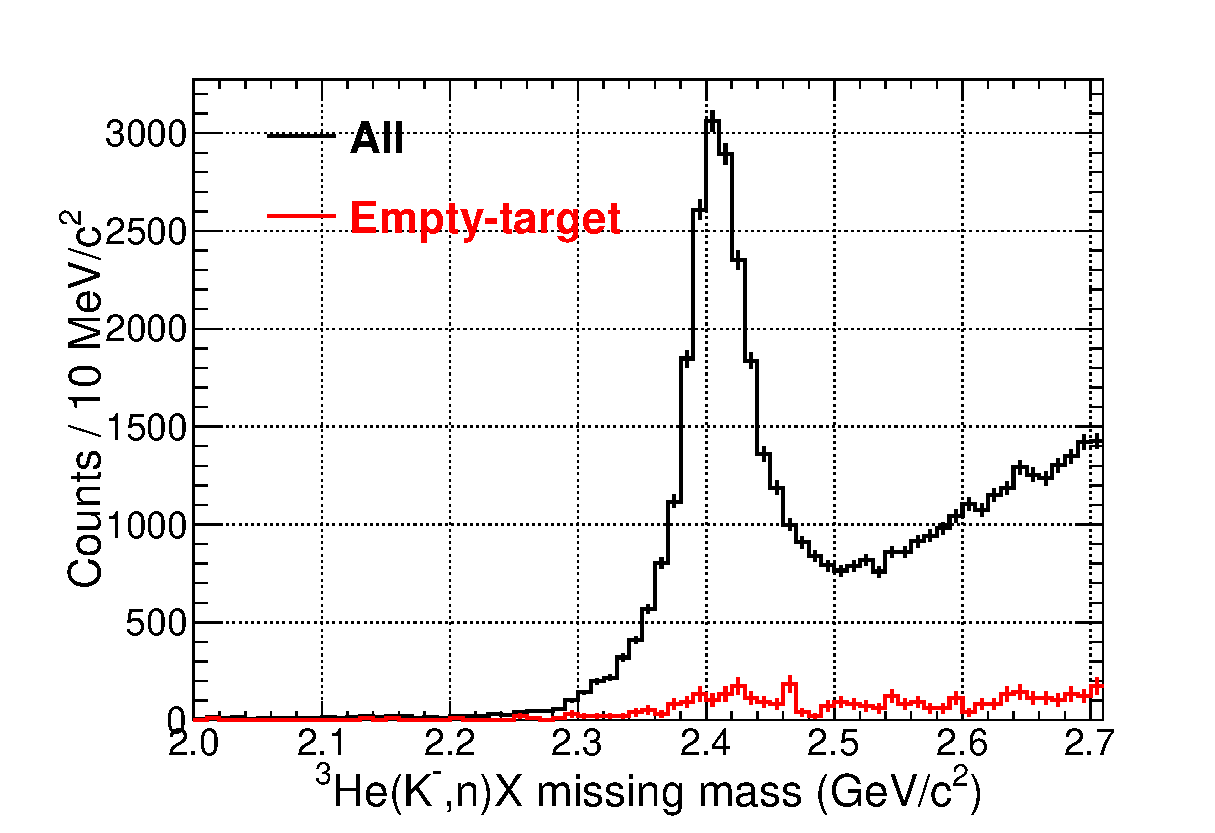
\includegraphics[width=12cm]{./fig/n-empty.eps}
\caption[Comparison between the $^3$He target data and the empty-target one.]{Comparison between the $^3$He target data and the empty-target one. The empty-target data is normalized by the kaon flux.}
\label{fig-nempty}
\end{center}
\end{figure}  

\subsubsection{Continuous background}
The yield of the purely accidental background can be assumed to be time constant and thus estimated from the $1/\beta$ spectrum as shown in Fig. \ref{fig-neutron}. However, the time-constant background is not enough to explain the yield even in unphysical region below the $\Lambda N$-mass threshold at 2054 MeV/$c^2$ in the missing mass spectrum as shown with green dotted line in Fig. \ref{fig-mmunphys}. To reproduce the yield in the unphysical region, we evaluate the background using an additional background whose shape is naturally expected to be smooth as an extrapolation from below the $\Lambda N$ threshold. Here we assume the continuous background is dominant at below 2.29 GeV/$c^2$, where no specific structures are expected. At above 2.29 GeV/$c^2$, the $Y^*N$ branches of non-mesonic two-nucleon absorption processes may contribute as discussed in Sec. \ref{sec-2na}.

We consider three shapes of the continuous background. The first one is assumed to be a purely time-constant distribution. The yield is determined by fitting the missing-mass spectrum with the time-constant background obtained with the $1/\beta$ spectrum. The second one is a combination of the time-constant background in 1/$\beta$ and a constant function in the missing-mass spectrum. The third one is similar to the second one but we employ a second-order polynomial function instead of the constant function. Their parameters are determined by fitting the the spectrum from 1.5 GeV/$c^2$ to 2.29 GeV/$c^2$. The resultant background shapes are shown in Fig. \ref{fig-mmunphys}. In the binding region, the background yield is evaluated to be less than 10\% of the total using any background.
\\

In summary, it is found that any experimental effect cannot explain the observed tail structure below the $K^-pp$ threshold; the tail structure cannot be reproduced by the detector resolution, the contamination from other materials than the target $^3$He, and the continuous backgrounds extrapolated from the unphysical region.

\begin{figure}[]
\begin{center}
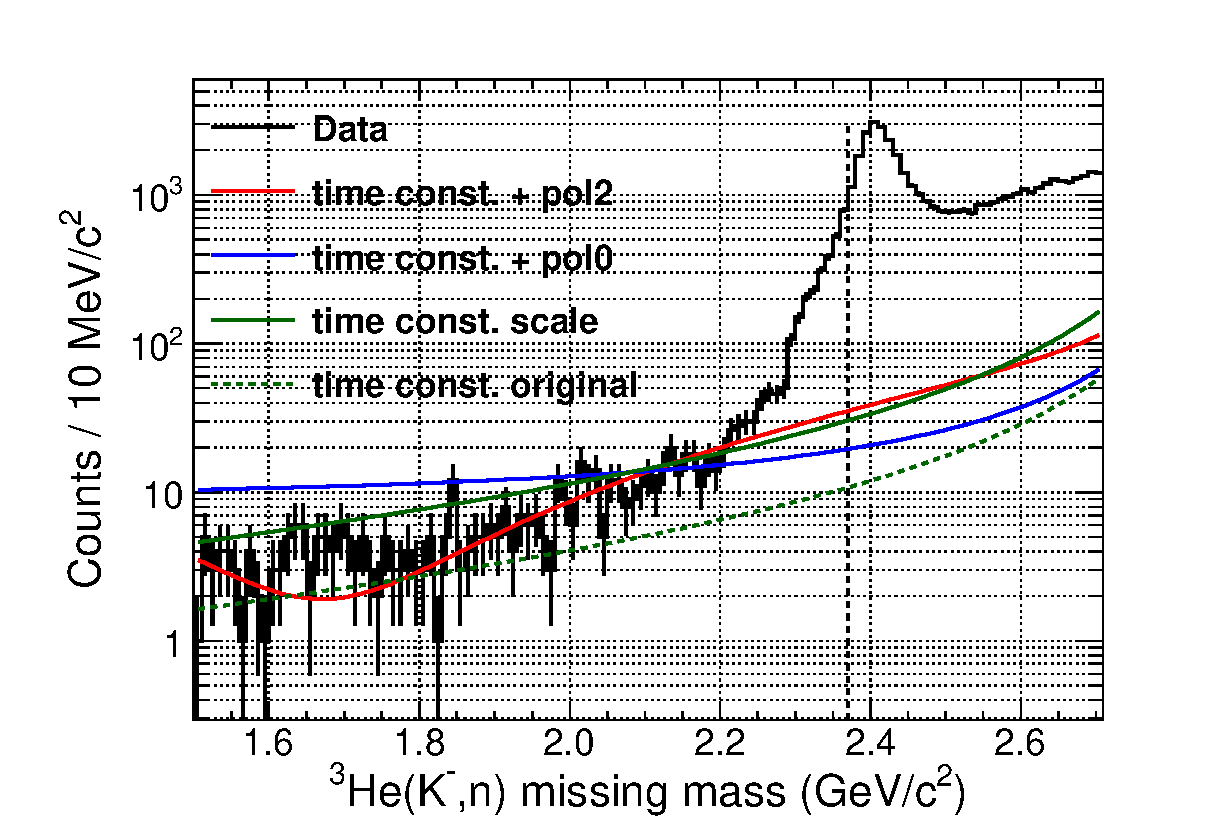
\includegraphics[width=12cm]{./fig/mm-unphys.eps}
\caption{Continuous background defined by the 3 types of assumptions.}
\label{fig-mmunphys}
\end{center}
\end{figure}  

\subsection{Contribution from the known single nucleon processes} \label{sec-global}
Now we consider known kaon-induced reactions from the previous experiments. Since there is very little information about the $K^-$+$^3$He reaction, direct comparison with previous data on the reaction is impossible. Instead, we examine the obtained missing-mass spectrum of $^3$He($K^-,n$)  using well-known elementally reactions of $K^-+p$ and $K^-+n$, which were measured mainly by hydrogen and deuterium bubble chamber experiments as the results are summarized in Table \ref{tab-kpreaction} and \ref{tab-knreaction}. In the deuterium bubble chamber experiments, some two-nucleon absorption reaction (2NA) processes, such as $K^- + d\to \Lambda(1405) + n$, were also observed. However, we focus on well-established elementally processes, i.e., single-nucleon ones. Discussion about the possible 2NA contributions is given in Sec. \ref{sec-2na}.

Figure \ref{fig-sim1n} shows the simulated neutron-spectrum for the known single-nucleon processes. They were generated by taking account of angular distributions of the reactions and the Fermi motion in $^3$He(see Fig. \ref{fig-geantfermi}). We simply assumed the total cross-section of the $K^-$-$^3$He reaction to be
\begin{eqnarray}
\sigma_{K^{-3}He} = 2 \times \sigma_{K^-p} + \sigma_{K^-n},
\end{eqnarray}
where $\sigma_{K^{-3}{\rm He}}$, $\sigma_{K^-p}$, and $\sigma_{K^-n}$ are the total cross-sections of $K^-$-$^3$He, p, and n reactions, respectively. Then we analyzed the simulated data in the same way as the experimental data. Details of the simulation can be found in Appendix A. 

The main features of the spectrum in Fig. \ref{fig-sim1n} are a peak structure just above the threshold and a bump structure in the larger missing mass region. These are qualitatively similar to the experimental spectrum (Fig. \ref{fig-ncs})\footnote{Although quantitative evaluation of the spectral shape above the $K^-pp$ threshold is difficult due to the uncertainty of nuclear effects in $^3$He, the results of the current analysis is not affected by such incompleteness of the simulation. This is because the well-known processes do not contribute the spectral shape below the threshold except for the $\Sigma$ productions, whose spectrum and yield are mainly evaluated using the experimental data.}.
The peak structure is so-called a quasi-free peak, which is composed of $K^-$ elastic reaction and charge exchange reaction as:
\begin{eqnarray*}
K^- + ^3\rm{He} &\to& K^- + n + p_s +p_s, \nonumber \\ 
K^- + ^3\rm{He} &\to& K^0 + n + d_s (p_s+n_s). \label{eq-k0}
\end{eqnarray*}
The contribution of these reactions to the $K^-pp$ bound region is not kinematically allowed as discussed in Sec. \ref{sec-exeff}. The bump structure is mainly due to hyperon decays.
Among them, only a decay neutron from $\Lambda$ and $\Sigma$ productions with one associated pion is kinematically allowed to produce fast neutrons which can contribute to the bound region. However, for the $\Lambda$ case such as, 
\begin{eqnarray*}
K^- + {\rm ^3He} &\to& \Lambda + \pi^0  + d_s (p_s+n_s),\\
&&\Lambda \to n + \pi^0,\\
K^- + {\rm ^3He} &\to& \Lambda + \pi^-  + p_s+ p_s,\\
&&\Lambda \to n + \pi^0,
\end{eqnarray*}
the simulation result shows the charged pion as well as the neutral one cannot be kinematically detected with the CDS in coincidence with the detection of the decay neutron with the NC. Therefore, such $\Lambda$ productions are expected not to contribute to the semi-inclusive $^3$He($K^-,n)X$ missing-mass spectrum. 
\\

In summary, it is found that only $\Sigma$ productions with one associated pion can contribute to the bound region. The contribution from these reactions is discussed in detail in the next section. 

\begin{figure}[]
\begin{center}
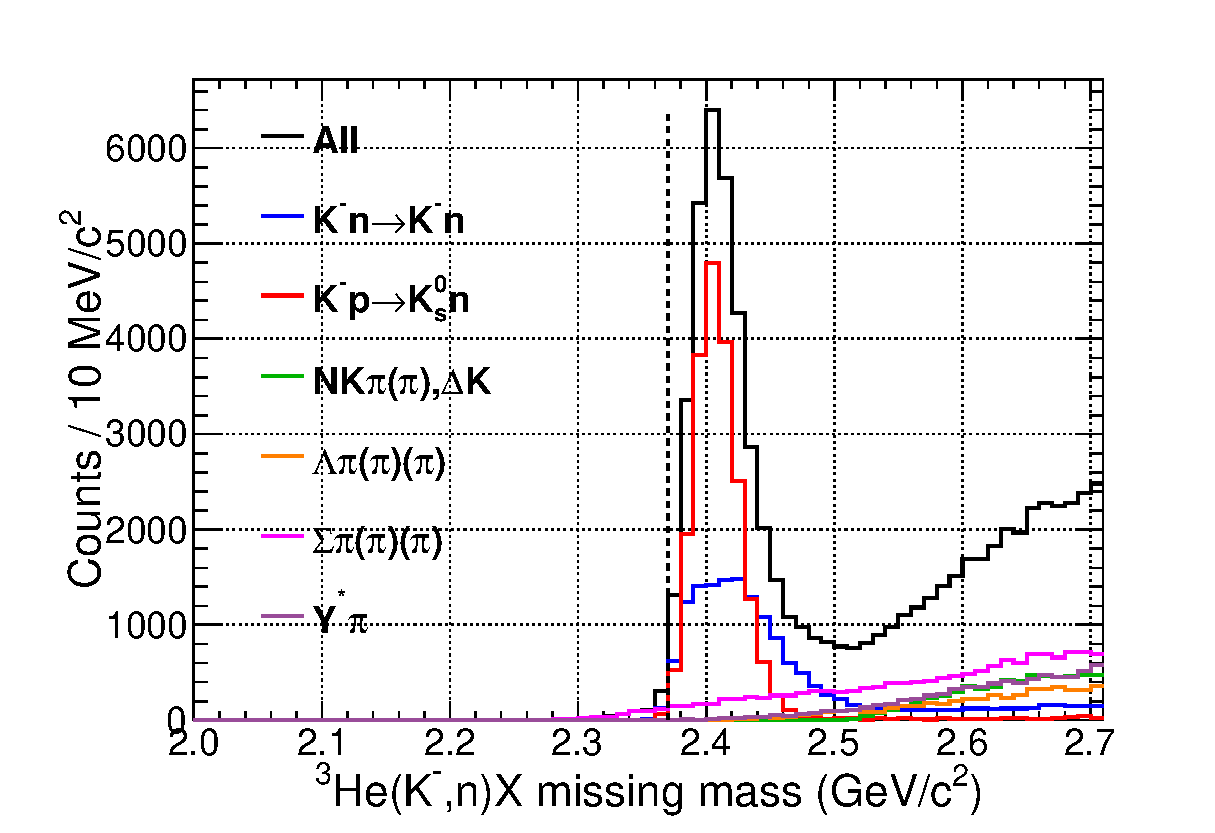
\includegraphics[width=12cm]{./fig/n-simk1n.eps}
\caption{Simulated neutron spectrum with the known elementally processes. }
\label{fig-sim1n}
\end{center}
\end{figure}  

\subsection{Contribution from $\Sigma$ decays \label{sec-sigmacut}}
Among the elementally processes, only $\Sigma$ productions with one associated pion are kinematically allowed to contribute to the bound region via their weak decays,
\begin{eqnarray}
K^- + {\rm ^3He} &\to& \Sigma^{\pm} + \pi^\mp_{prod} + d_s(p_s+n_s), \label{eq-sigma}\\
&&\Sigma^\pm \to n + \pi^\pm_{decay}, \nonumber \\
K^- + {\rm ^3He} &\to& \Sigma^{-} + \pi^0_{prod} + p_s + p_s, \label{eq-sigma2}\\
&&\Sigma^- \to n + \pi^-_{decay}, \nonumber
\end{eqnarray}
where $\pi_{prod}$ and $\pi_{decay}$ denote the associated pion in the reactions and the decay pion from $\Sigma$, respectively. The $\Sigma$ decays are reconstructed from the forward-going neutron detected with the NC and the $\pi_{decay}$ detected with the CDS as shown in Fig. \ref{fig-sigmaraw}. In particular, a fast neutron is generated as a decay product of forward-going $\Sigma$ in these reactions. In such case, $\pi_{prod}$ is mostly emitted backward and often out of the CDS acceptance, while at least one of $\pi_{prod}$ and $\pi_{decay}$ must be detected with the CDS to be triggered. Therefore the $\Sigma$ reconstruction efficiency $\epsilon^{\Sigma}_{reconstruct}$, which is defined as,
\begin{eqnarray*}
\epsilon^{\Sigma}_{reconstruct}=\frac{\rm( Number\ of\ reconstructed\ \Sigma s\ with\ neutrons\ in\ the\ bound\ region)}{\rm (Number\ of\ reconstructed\ neutrons\ in\ the\ bound\ region\ from\ \Sigma\ decays)}
\end{eqnarray*}
is expected to be rather high.

In the following, the $\Sigma$-decay contribution to the bound region is evaluated using the experimental data with $\epsilon^{\Sigma}_{reconstruct}$ obtained by the simulation. 

\subsubsection{$\Sigma$ reconstruction efficiency} \label{sec-sigma}
A realistic evaluation of the efficiency $\epsilon^{\Sigma}_{reconstruct}$ was performed in the same frame work of the simulation described in Sec. \ref{sec-global}. Figure \ref{fig-sigmasimdist}(left) shows the simulated correlation between the $\pi_{decay}$ (not required to be detected) angle in the laboratory system and the neutron missing mass when the neutron is detected with the NC. Most of fast-neutron events, corresponding to the missing-mass of below the $K^-pp$ binding threshold, involve $\pi_{decay}$ of within the CDH acceptance, $|\cos\theta_{\pi_{decay}}|<\sim$0.6. Figure \ref{fig-sigmasimdist}(right) shows the angular distribution of $\pi_{decay}$ with requiring the decay neutron to be detected with the NC and its missing mass of $^3$He($K^-,n)X$ to be smaller than the $K^-pp$ binding threshold. In the figure, the black, red, and blue histograms represent the generated, the charged-particle tagged, and the $\Sigma$ reconstructed events, respectively. Then the efficiency $\epsilon^{\Sigma}_{reconstruct}$ can be calculated as the ratio of the blue histogram to the red one, and was obtained to be $\sim$90\% as summarized in Table \ref{tab-sigmacut}. Here the $\Sigma^\pm$ signal region was defined as $|$IM(n$\pi^\pm)-m_{\Sigma^\pm}$$|<$ 12 MeV/$c^2$, which corresponds to about $\pm2 \sigma$ of the invariant mass resolution.

\begin{figure}[]
\begin{center}
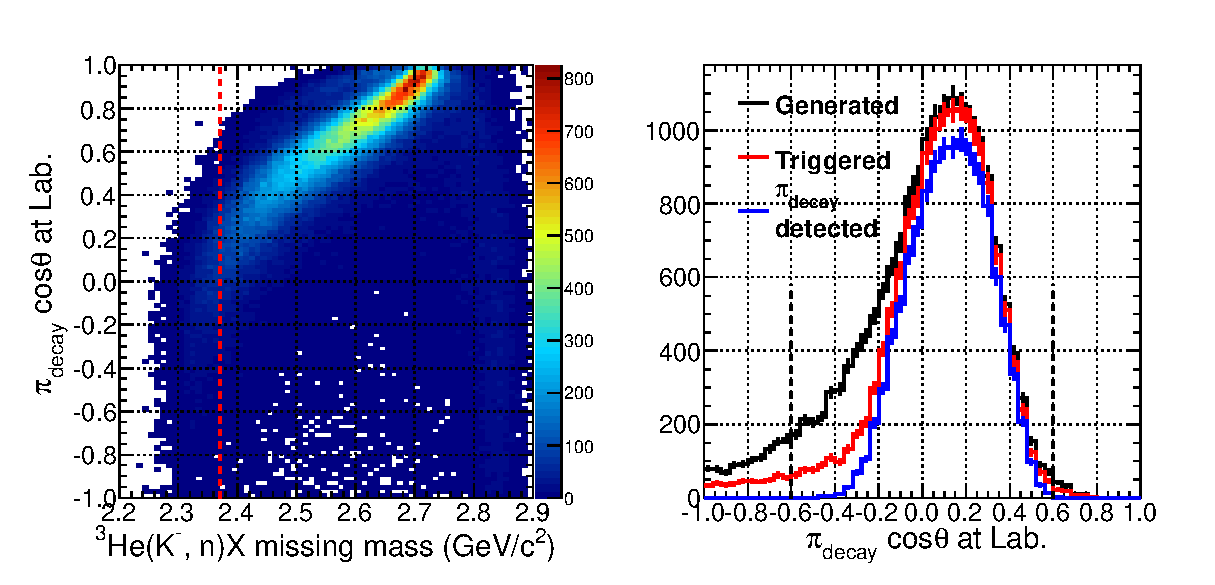
\includegraphics[width=\columnwidth]{./fig/sigma-simdist.eps}
\caption[Simulated $\pi_{decay}$ distributions in the $\Sigma$ productions.]{(left) Simulated correlation between the $\pi_{decay}$ angle and the neutron missing-mass in the $\Sigma$ productions. The dotted red line represents the $K^-pp$ binding threshold. (right) Simulated angle distribution of pions from $\Sigma$ decays. The decay neutrons are requested to be detected with the NC and the below $K^-+p+p$ threshold. The dotted lines represents the CDH acceptance. A part of pions can not reach the CDH because of their low momenta. }
\label{fig-sigmasimdist}
\end{center}
\end{figure}  

\begin{table}[]
\caption[$\Sigma$ reconstruction efficiencies obtained by the simulation.]{$\Sigma$ reconstruction efficiencies obtained by the simulation. The errors are statistical ones.}
\begin{center}
\begin{tabular}{l|c}
\hline\hline
Channel & $\epsilon^\Sigma_{reconstruction}$ (\%)\\
\hline
$K^- + {\rm ^3He} \to \Sigma^{+} + \pi^- + d_s$  & 85 $\pm$ 1 \\
$K^- + {\rm ^3He} \to \Sigma^{-} + \pi^+ + d_s$  & 91 $\pm$ 1 \\
$K^- + {\rm ^3He} \to \Sigma^{-} + \pi^0 + p_s + p_s$ & 91 $\pm$ 1 \\
\hline\hline
\end{tabular}
\end{center}
\label{tab-sigmacut}
\end{table}%

\subsubsection{Identification and removal of the $\Sigma$-decay events} 
By reconstructing the $\Sigma$ decays as described above, the decay neutron can be identified event by event. Figure \ref{fig-sigmadatacut1}(left) shows the correlation between the $n\pi^-$ invariant mass and the neutron missing mass. A narrow band can be seen in the horizontal direction at the mass of $\Sigma^-$, while there is also an event concentration in the vertical direction attributed to the charge-exchange reactions $K^-p\to K^0_sn$, followed by the the $K^0_s\to\pi^+\pi^-$. Therefore, selected $\Sigma$-decay events contain the quasi-free events to some extent as shown in Fig. \ref{fig-sigmadatacut1}(right). 

Figure \ref{fig-ncswosigma} shows the $^3$He($K^-,n)X$ missing mass spectrum after the removal of $\Sigma$-decay events. The tail structure below the threshold is kept in a similar shape as shown in Fig. \ref{fig-ncs}. Although there still remains little contribution from the $\Sigma$-decay events due to the $\sim$10\% inefficiency of the $\Sigma$ reconstruction, it obviously does not destroy the tail structure. %The spectrum after the removal of neutrons from $\Sigma$ decays is used in the following discussions.
\begin{figure}[]
\begin{center}
\includegraphics[width=\columnwidth]{./fig/sigma-datacut1.eps}
\caption[Contributions of the $\Sigma$-decay events. ]{(left) Correlation between the n$\pi^-$ invariant mass and the neutron missing mass obtained from the experimental data. The horizontal solid lines represent the $\Sigma$ selection regions, and the red dotted line represents $K^-pp$ binding threshold. (right) Contributions of the $\Sigma$-decay events in the neutron missing-mass spectrum.}
\label{fig-sigmadatacut1}
\end{center}
%\end{figure}  
%\begin{figure}[]
\begin{center}
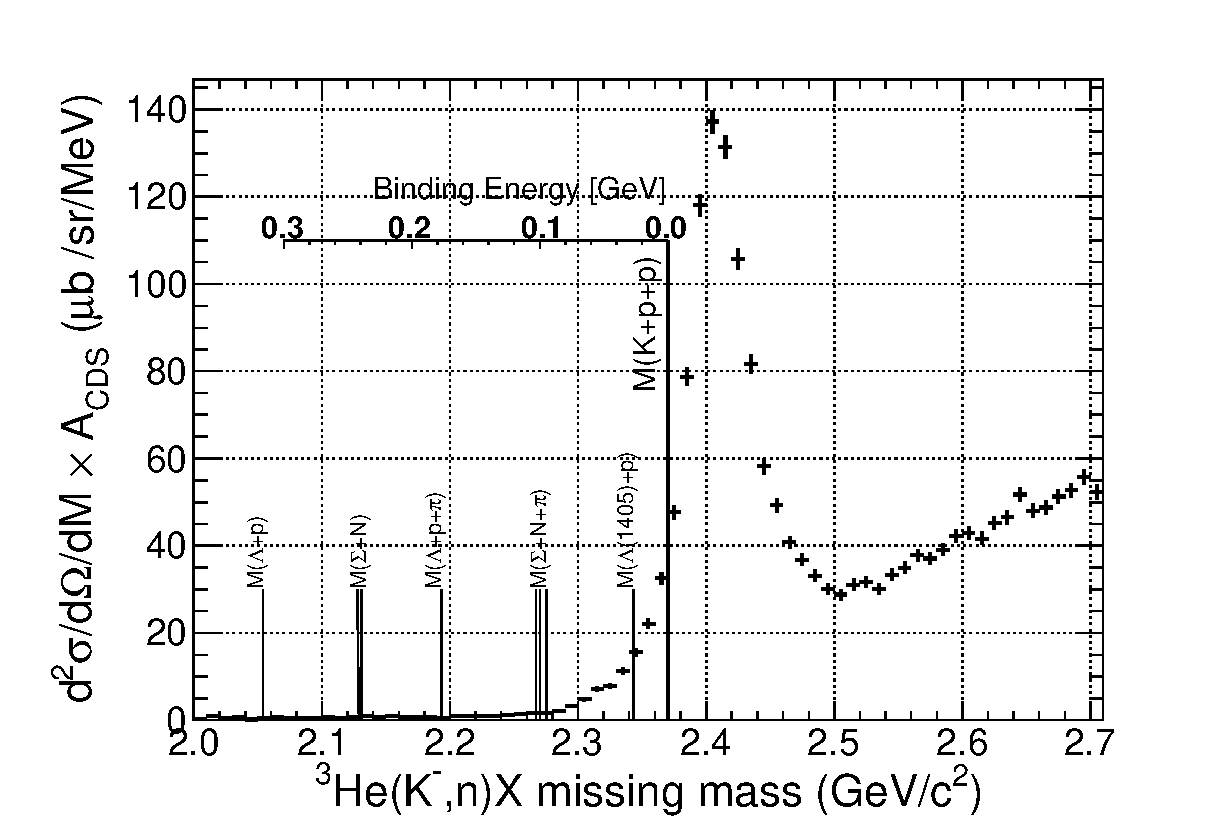
\includegraphics[width=12cm]{./fig/n-cswosigma1.eps}
\caption{Neutron missing mass spectrum after the removal of $\Sigma$-decay events.}
\label{fig-ncswosigma}
\end{center}
\end{figure}  

\subsection{Yield estimation of the unknown excess}
Figure \ref{fig-nbg} shows the $^3$He($K^-,n)X$ missing-mass spectrum with each contribution from the experimental effects and the well-known single-nucleon processes discussed above, where we employ the $K^0_s$-tagged spectrum for the main component of the quasi-free peak. $\Sigma$-decay events were already removed event by event in each contribution. It is obvious that the tail structure below the threshold cannot be reproduced by any experimental effect nor well-established elementary-process. 

Then, we evaluated the yield of the excess in the bound region using the spectra. The integrated region was set from 2.29 to 2.37 GeV/$^c$, since continuous background should be dominant below the region. The excess-yield in the region of the interest is obtained to be 1462 $\pm$ 58(stat.) $\pm $122(syst.), while the sum of the backgrounds is 568 $\pm$ 57(stat.) $\pm$ 121(syst.). The yields of each component are summarized in Table \ref{tab-bound}. The evaluations of their associated errors are as follow.
 
\begin{figure}[]
\begin{center}
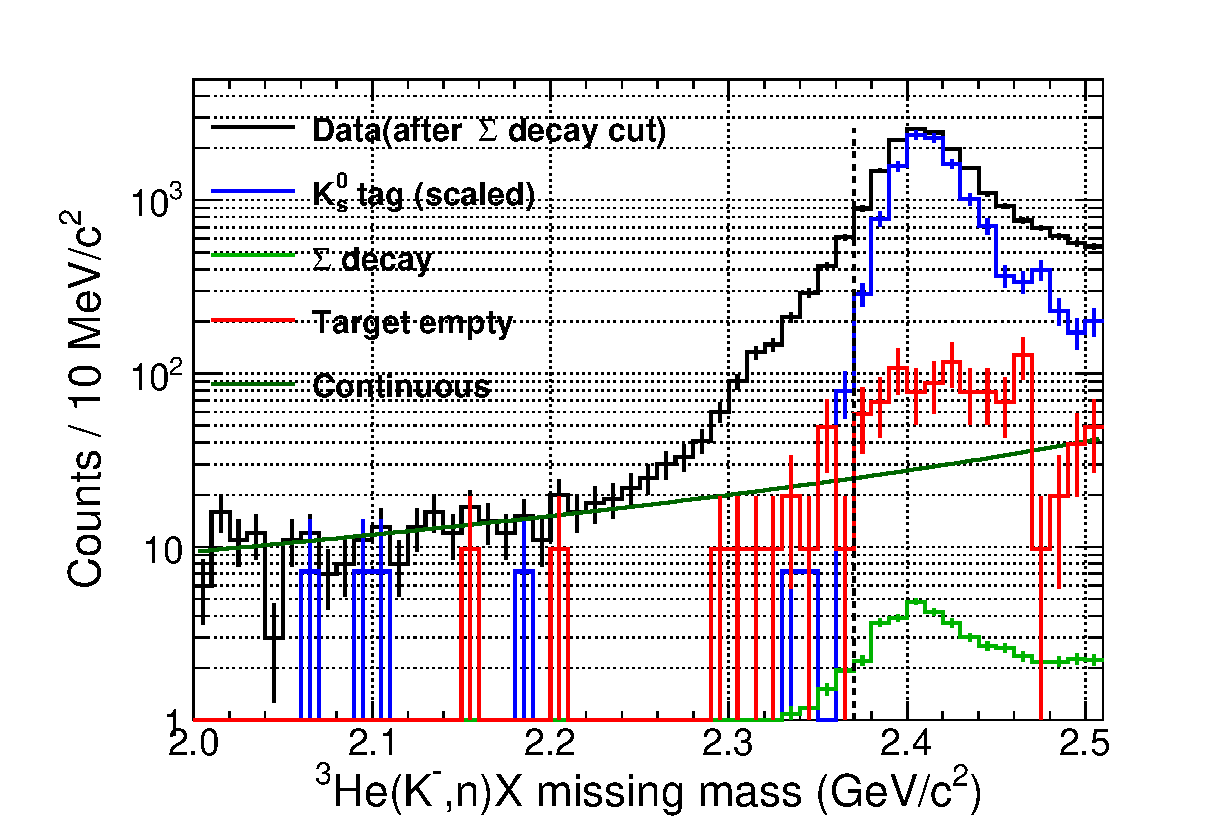
\includegraphics[width=12cm]{./fig/n-bg.eps}
\caption{Summary plot of the experimental effects and the known processes. }
\label{fig-nbg}
\end{center}
\end{figure}  

\begin{table}[]
\caption{Obtained yields in the bound region.}
\begin{center}
\begin{tabular}{llcccc} 
\hline\hline										
	&		&	Count	&	stat.	&	syst.	&	syst.  from	\\
	&		&		&	error	&	error	&	energy scale	\\
\hline											
Total event	&		&	2030	&	45	&		&	212	\\
\hline											
Background	&	total	&	568	&	57	&	60	&	105	\\
\hline										
	&	Continuous	&	197	&	14	&	47	&	2	\\
	&	~~(time const. only)	&	199	&	14	&		&		\\
	&	~~(time const. + pol0)	&	150	&	12	&		&		\\
	&	~~(time const. + pol2)	&	243	&	16	&		&		\\
	&	Target-empty	&	134	&	37	&	13	&	30	\\
	&	$\Sigma$-decay event	&	82	&	9	&	16	&	5	\\
											
	&	Quasi-free tail	&	155	&	40	&	31	&	83	\\
\hline																																
Unknown	&		&	1462	&	58	&	60	&	107	\\
\hline\hline									
\end{tabular}
\end{center}
\label{tab-bound}
\end{table}%
\subsubsection{Contamination of quasi-free peak}
The main component of the quasi-free peak, namely contributions from the kaon charge exchange reaction and the kaon elastic scattering, should appear only above the $K^-pp$ threshold because of their kinematics as already discussed. However, the finite experimental resolution makes them contribute in the bound region. Here the $K^0_s$ tagged spectrum is scaled to fit the peak height for the estimation of such contribution. The uncertainty in the assumption, i.e. the shape of the quasi-free peak can be substituted by the $K^0_s$-tagged spectrum, is evaluated to be 20\%.

\subsubsection{Continuous background}
We have defined three types of the continuous background as shown in Fig. \ref{fig-mmunphys}. Their average is adopted in the yield estimation and the difference among them is considered as a systematic error.

\subsubsection{Contributions from other materials than $^3$He}
The uncertainty of the contribution from other materials than $^3$He is due to that of the total kaon flux. Since the empty-target data was analyzed with the same procedure as used in the production-data analysis, the uncertainty is almost the same as that of the production-data evaluated to be $\sim$2\% as summarized in Table \ref{sec-luminosity}. However, an additional systematics should arise because the empty-target data was taken in a different accelerator cycle with lower beam intensity. Therefore, we conservatively adopted a 10\% systematic error here.

\subsubsection{Neutrons from $\Sigma$ decays}
In the discussion on the removal of the  $\Sigma$-decay events described in Sec. \ref{sec-sigma}, it is found that $\sim$10\% neutrons from the $\Sigma$ decays are failed to be reconstructed. Here we assume the spectral shape of those events is the same as that of reconstructed events. The $\Sigma^-$ can be produced via reaction \ref{eq-sigma} and \ref{eq-sigma2}. The ratio of the two reaction is assumed to be (Eq. \ref{eq-sigma}):(Eq. \ref{eq-sigma2})=3:1, by taking account of the elementary cross sections (Table \ref{tab-kpreaction},\ref{tab-knreaction}) and the number of each nucleon in $^3$He. Conservatively, 10\% systematic error arises from the uncertainty of the reconstruction inefficiency of $\Sigma$. The uncertainty in the estimation method is evaluated to be 20\% in total.

\subsubsection{Uncertainty in the missing mass scale}
Systematic errors arising from the uncertainty in the absolute missing mass scale are evaluated by shifting the integral gate. Note that the large errors of the total and the quasi-free tail are due to the rise of the spectrum near the $K^-pp$ threshold.
\\

\subsection{Conclusion on the tail structure in the $K^-pp$ bound region}
The experimental effects and well-established processes are examined focusing on their contributions to the $^3$He($K^-.n)X$ missing-mass spectrum below the $K^-pp$ threshold. Consequently, it is found that the contributions are much smaller than the strength of the observed tail structure. The yield of the unknown excess is evaluated to be 1462 $\pm$ 58(stat.) $\pm $ 122(syst.), while that of the experimental backgrounds and well-known processes is to be 568 $\pm$ 57(stat.) $\pm$ 121(syst.) events, by integrating the spectra from 2.29 to 2.37 GeV/$c^2$. Thus the observed excess is statistically significant,  and the result is robust against the systematics arising from the analysis procedure.

The unknown excess was successfully observed as we aimed at by employing the $^3$He($K^-,n$) reaction to kinematically separate the known background processes and by constructing new spectrometer system to achieve good experimental resolution and to suppress the unphysical backgrounds. The unknown events must have total baryon number 2 and strangeness -1 to be consistent with the $^3$He($K^-,n$) reaction. Such structure just below the $K^-pp$ threshold was observed by the present experiment for the first time. 
